\documentclass{article}
\usepackage[utf8]{inputenc}
\usepackage{datetime}
\usepackage{enumerate}
\usepackage{textcomp}
\usepackage{amsmath}
\usepackage{amssymb}
\usepackage[edges]{forest}
\usepackage{tikz}
\usetikzlibrary{shapes, backgrounds, automata, positioning, arrows}
\usetikzlibrary{arrows}
\usepackage{listings}

\usepackage{titlesec}
\newcommand{\sectionbreak}{\clearpage}

\title{\bf \Large ASSIGNMENT 10}
\author{Xinhao Luo} 
\date{\today}

\def\math#1{$#1$}

\setlength{\textheight}{8.5in}
\setlength{\textwidth}{6.5in}
\setlength{\oddsidemargin}{0in}
\setlength{\evensidemargin}{0in}
\voffset0.0in

\usepackage{pifont}% http://ctan.org/pkg/pifont
\newcommand{\cmark}{\text{\ding{51}}}
\newcommand{\xmark}{\text{\ding{55}}}

\begin{document}
\maketitle
\medskip

\section{DMC Problem 25.8(f)}
\begin{enumerate}[i)]
    \item \math{S \to A0A}
    \item \math{A \to 0A1\vert 1A0\vert AA \vert 0A \vert \varepsilon}
\end{enumerate}

\section{DMC Problem 26.5(d)}
\begin{enumerate}[i)]
    \item Pseudo Code
        \begin{enumerate}[1)]
            \item Check if the string is valid (not empty, no 1 included), and mark the first bit with \xmark
            \item Back to \xmark, check if all bits after \xmark are marked
                \begin{itemize}
                    \item If True, ACCEPT
                    \item Otherwise, move back to \xmark
                \end{itemize}
            \item Move right and find the next non-marked bit, mark it
                \begin{itemize}
                    \item If \textvisiblespace, REJECT
                \end{itemize}
            \item Move right the next non-mark bit, and goto step 3
                \begin{itemize}
                    \item If \textvisiblespace, go to step 2
                \end{itemize}
        \end{enumerate}
    \item Machine Code
        \begin{enumerate}[1)]
            \item 
                \begin{figure}[ht] % ’ht’ tells LaTeX to place the figure ’here’ or at the top of the page
                    \centering % centers the figure
                    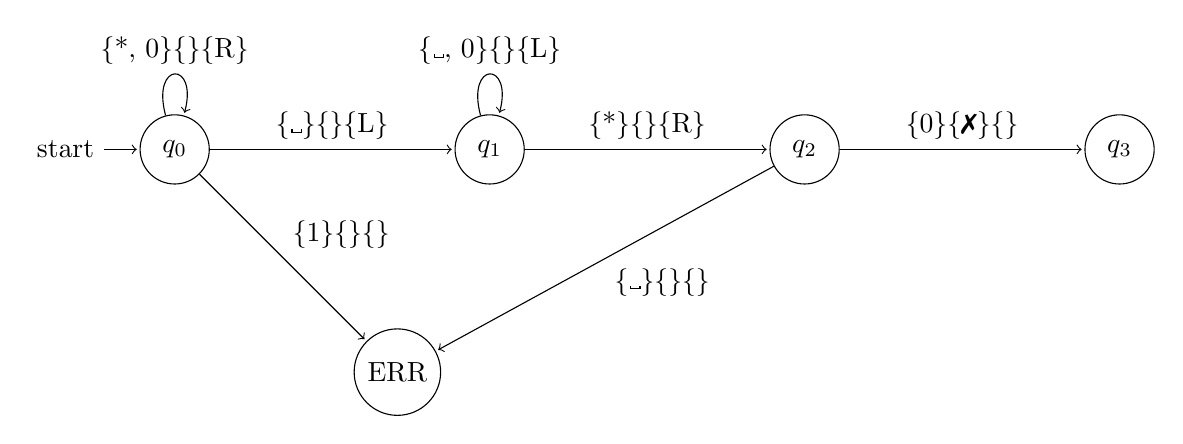
\begin{tikzpicture}[shorten >=1pt,node distance=4cm,on grid,auto] 
                       \node[state,initial] (q_0) {\math{q_0}}; 
                       \node[state] (q_1) [right=of q_0] {\math{q_1}}; 
                       \node[state] (q_2) [right=of q_1] {\math{q_2}}; 
                       \node[state] (q_3) [below right=of q_0] {ERR};
                       \node[state] (q_4) [right=of q_2] {\math{q_3}};
                    %   \node[state, accepting] (q_8) [below right=of q_6] {\math{q_8}};
                       \path[->] 
                        (q_0) edge [loop above] node {\{*, 0\}\{\}\{R\}} ()
                        (q_0) edge node {\{\textvisiblespace\}\{\}\{L\}} (q_1)
                        (q_0) edge node {\{1\}\{\}\{\}} (q_3)
                        (q_1) edge [loop above] node {\{\textvisiblespace, 0\}\{\}\{L\}} ()
                        (q_1) edge node {\{*\}\{\}\{R\}} (q_2)
                        (q_2) edge node {\{\textvisiblespace\}\{\}\{\}} (q_3)
                        (q_2) edge node {\{0\}\{\xmark\}\{\}} (q_4);
                    \end{tikzpicture}
                    \caption{Step 1}
                    \label{STEP1}
                \end{figure}
            \item 
                 \begin{figure}[ht] % ’ht’ tells LaTeX to place the figure ’here’ or at the top of the page
                    \centering % centers the figure
                    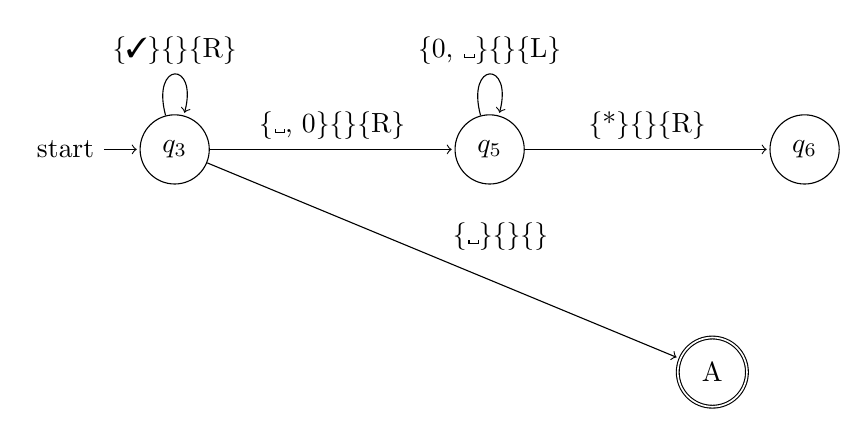
\begin{tikzpicture}[shorten >=1pt,node distance=4cm,on grid,auto] 
                       \node[state,initial] (q_4) {\math{q_3}}; 
                       \node[state] (q_5) [right=of q_4] {\math{q_5}}; 
                       \node[state] (q_6) [right=of q_5] {\math{q_6}}; 
                       \node[state, accepting] (q_8) [below right=of q_5] {A};
                       \path[->] 
                        (q_4) edge [loop above] node {\{\cmark\}\{\}\{R\}} ()
                        (q_4) edge node {\{\textvisiblespace\}\{\}\{\}} (q_8)
                        (q_4) edge node {\{\textvisiblespace, 0\}\{\}\{R\}} (q_5)
                        (q_5) edge [loop above] node {\{0, \textvisiblespace\}\{\}\{L\}} ()
                        (q_5) edge node {\{*\}\{\}\{R\}} (q_6);
                    \end{tikzpicture}
                    \caption{Step 2}
                    \label{STEP2}
                \end{figure}
        \end{enumerate}
    \item 
         \begin{figure}[ht] % ’ht’ tells LaTeX to place the figure ’here’ or at the top of the page
            \centering % centers the figure
            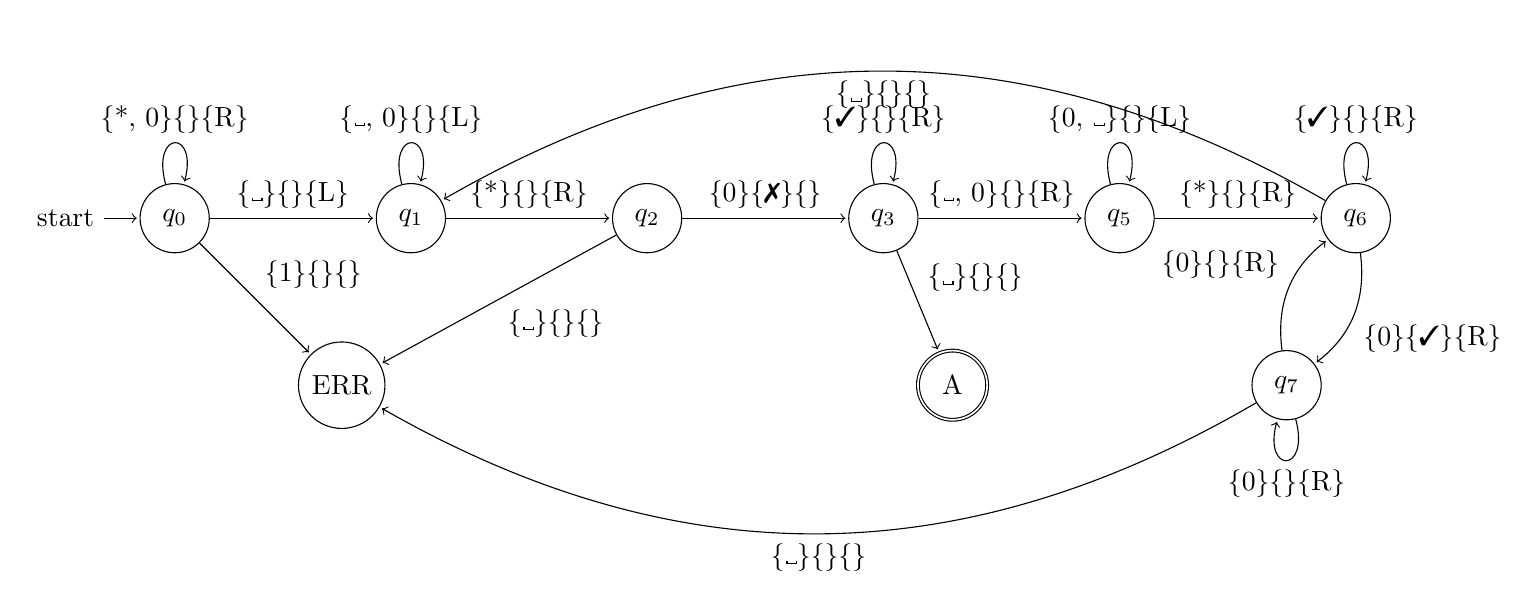
\begin{tikzpicture}[shorten >=1pt,node distance=3cm,on grid,auto] 
               \node[state,initial] (q_0) {\math{q_0}}; 
               \node[state] (q_1) [right=of q_0] {\math{q_1}}; 
               \node[state] (q_2) [right=of q_1] {\math{q_2}}; 
               \node[state] (q_3) [below right=of q_0] {ERR};
               \node[state] (q_4) [right=of q_2] {\math{q_3}};
               \node[state] (q_5) [right=of q_4] {\math{q_5}}; 
               \node[state] (q_6) [right=of q_5] {\math{q_6}};
               \node[state] (q_7) [below right=of q_5] {\math{q_7}}; 
               \node[state, accepting] (q_8) [below left=of q_5] {A};
            %   \node[state, accepting] (q_8) [below right=of q_6] {\math{q_8}};
               \path[->] 
                (q_0) edge [loop above] node {\{*, 0\}\{\}\{R\}}
                (q_0) edge node {\{\textvisiblespace\}\{\}\{L\}} (q_1)
                (q_0) edge node {\{1\}\{\}\{\}} (q_3)
                (q_1) edge [loop above] node {\{\textvisiblespace, 0\}\{\}\{L\}}
                (q_1) edge node {\{*\}\{\}\{R\}} (q_2)
                (q_2) edge node {\{\textvisiblespace\}\{\}\{\}} (q_3)
                (q_2) edge node {\{0\}\{\xmark\}\{\}} (q_4)
                (q_4) edge [loop above] node {\{\cmark\}\{\}\{R\}}
                (q_4) edge node {\{\textvisiblespace\}\{\}\{\}} (q_8)
                (q_4) edge node {\{\textvisiblespace, 0\}\{\}\{R\}} (q_5)
                (q_5) edge [loop above] node {\{0, \textvisiblespace\}\{\}\{L\}}
                (q_5) edge node {\{*\}\{\}\{R\}} (q_6)
                (q_6) edge [bend left] node {\{0\}\{\cmark\}\{R\}} (q_7)
                (q_7) edge [bend left] node {\{0\}\{\}\{R\}} (q_6)
                (q_6) edge [loop above] node {\{\cmark\}\{\}\{R\}} ()
                (q_7) edge [loop below] node {\{0\}\{\}\{R\}} ()
                (q_7) edge [bend left] node {\{\textvisiblespace\}\{\}\{\}} (q_3)
                (q_6) edge [bend right] node {\{\textvisiblespace\}\{\}\{\}} (q_1);
            \end{tikzpicture}
            \caption{Final Version}
            \label{Final}
        \end{figure}
\end{enumerate}

\section{DMC Problem 26.8(f)}
\begin{enumerate}[1)]
    \item Move right to the first non-marked bit, mark it and remember it.
        \begin{itemize}
            \item if \textvisiblespace, return to \text{*}; erasing all marks and halt
        \end{itemize}
    \item Move right to the last non-marked bit
        \begin{itemize}
            \item If there is none, return to \text{*}, erasing all marks and halt
            \item Otherwise, remember it, replace it with the bit from step 1 and mark it
        \end{itemize}
    \item Move left to the first marked bit
        \begin{itemize}
            \item Replace the bit with the bit remembered in step 2 and goto step 1
        \end{itemize}
\end{enumerate}

\section{DMC Problem 27.4(b)}
Define function "Debugger(FUNCTION[, INPUT])", where INPUT is an optional input for the function, and it will return True when given function will halt with given input, False otherwise.
\begin{lstlisting}
def findNext(i):
    if i is Prime and i + 2 is prime:
        return i
    else:
        findNext(i + 1)

def test():
    for j in Prime Number Set:
        if Debugger(findNext, j) is False:
            break
\end{lstlisting}

If statement "Debugger(test)" return True, then it proves that the number of twin prime is infinite; otherwise there will be finite number of pairs. 

\section{DMC Problem 27.20}
\begin{enumerate}[a)]
    \item B is also undecidable
    \item Unsure about B
    \item Unsure about A
    \item A is decidable
\end{enumerate}


\section{DMC Problem 27.45}
\begin{enumerate}[a)]
    \item \math{3 \cdot d_1 + 4 \cdot d_2}
    \item \math{d_1 \cdot 2 + d_3 + d_4 \cdot 2 + d_2 \cdot 2}
\end{enumerate}

\section{DMC Problem 27.46}
If each domino has the same content on both top and bottom, it doesn't really matter what sequence or number of domino used, as it will always be a solution. \\
Input Format: \math{\alpha_1\#\alpha_2...\#\#\delta_1\#\delta_2...} \\
The sketch of the Turing machine is shown below:

INPUT: \textless S\textgreater The encoded domino strings.
\begin{enumerate}
    \item Check that \textless S\textgreater is a valid encoding of dominoes set
    \item Back to beginning; find and mark (\cmark) the first unmarked bit from the beginning and remember it
        \begin{itemize}
            \item If \#, goto step 8
            \item If \textvisiblespace, REJECT
        \end{itemize}
    \item Move right to find the double pun, and stop at the first pun
    \item Move right and find the first unmarked bit
        \begin{itemize}
            \item If the bit does not match the one in step 2, continue to step 5
            \item If matched, mark (\cmark) it and move to step 2
        \end{itemize}
    \item Move right and mark the rest of the string with \xmark until a pun is met
    \item Move to beginning, and find the first non-marked bit
    \item Move right and mark the rest of the string with \xmark until a pun is met, then goto step 2
    \item Move left, and check if string before before a pun or * was met has all marked (\cmark)
        \begin{itemize}
            \item If true, ACCEPT
            \item Otherwise, go back to step 2
        \end{itemize}
\end{enumerate}

\end{document}